%-------------------------------------------------------------------------------
% 								BAB I
% 							LATAR BELAKANG
%-------------------------------------------------------------------------------

\chapter{PENDAHULUAN}

\section{Latar Belakang}
Ibu kota provinsi Aceh yaitu Banda Aceh, memiliki kawasan bernama Kopelma (Kota Pelajar Mahasiswa) dimana terdapat dua perguruan tinggi yang menjadi kebanggaan masyarakat Aceh yaitu Universitas Syiah Kuala (Unsyiah) dan Universitas Islam Negeri (UIN) Ar-Raniry. Sehingga Banda Aceh menjadi tempat favorit bagi calon mahasiswa yang ingin melanjutkan studi. Bukan hanya dari daerah-daerah di Aceh saja, namun masyarakat luar Aceh juga sudah mulai melirik Banda Aceh sebagai kota destinasi tempat pendidikan mereka \citep{abduh2016}. Berdasarkan informasi yang disampaikan melalui portal data Universitas Syiah Kuala (Unsyiah), jumlah mahasiswa aktif pada tahun 2017 mencapai 25.547 mahasiswa. Berdasarkan buku Statistik Banda Aceh 2017, jumlah mahasiswa aktif UIN Ar-Raniry pada tahun 2016 mencapai 17.804 mahasiswa \citep{bappeda2017}. Belum lagi jumlah mahasiswa dari PTN dan PTS lainnya yang berada di Banda Aceh. Gambar \ref{spandukkos} adalah contoh spanduk kos-kosan.
\begin{figure}[H]
	\centering
	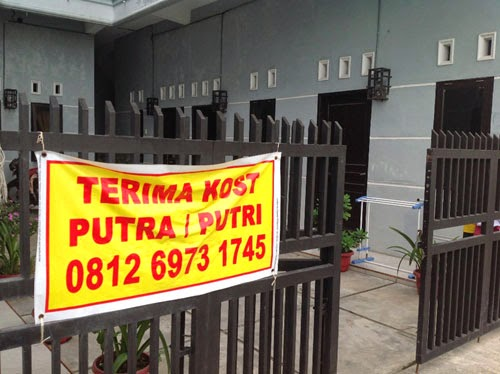
\includegraphics[scale=0.5]{gambar/spandukkos}
	\caption{Spanduk penerimaan kos.}
	\label{spandukkos}
\end{figure}
Peningkatan jumlah mahasiswa di Kota Banda Aceh setiap tahunnya ini, menyebabkan kebutuhan akan informasi mengenai tempat kos pun menjadi semakin meningkat. Meningkatnya jumlah mahasiswa di Kota Banda Aceh menimbulkan persaingan di antara mahasiswa untuk mencari tempat tinggal sementara seperti kos. Berdasarkan hasil diskusi dengan pencari kos, ada beberapa cara untuk mendapatkan informasi mengenai kos-kosan, antara lain adalah melihat rumah yang terdapat pamplet atau brosur bertuliskan terima kos, brosur di persimpangan jalan, informasi dari teman atau kerabat, informasi kosan dari \textit{broadcast} aplikasi \textit{chatting}, dari sosial media dan lain-lain. Informasi dari pamplet atau brosur akan mengeluarkan biaya yang berulang-ulang untuk pembuatan pamplet maupun brosur yang mudah rusak akibat kondisi cuaca hujan, angin, atau bahkan dicabut oleh oknum jahil.  Informasi dari \textit{broadcast} aplikasi \textit{chatting} bisa mendapatkan informasi yang tidak \textit{update} bahkan \textit{hoax}. 

Sebagai mahasiswa yang berasal dari luar Banda Aceh dan belum memiliki tempat tinggal, mencari tempat kos adalah salah satu hal yang difikirkan. Belum mengenal wilayah Banda Aceh menjadi salah satu kendala bagi orang yang baru pertama kali mengunjungi Banda Aceh untuk mencari kos. Sehingga pencari kos membutuhkan cara yang dapat memberikan informasi lengkap mulai dari fasilitas yang tersedia hingga harga kos, tanpa perlu menghabiskan waktu untuk mendatangi tempat kos satu persatu dan bertanya langsung kepada pemilik kos. 

Oleh karena itu, berdasarkan uraian di atas perlu dikembangkan aplikasi berbasis Android, dimana pencari kos dapat mencari kos yang berada di Kota Banda Aceh dan sekitarnya sesuai kebutuhan dan aplikasi ini akan menampilkan informasi mengenai kos tersebut. Selain mencari kos melalui aplikasi, bagi pencari kos yang masih berkeliling Kota Banda Aceh untuk mendapatkan kos, dapat memanfaatkan fitur \textit{Scanner} kode QR (\textit{Quick Reference}). Jika pencari kos menemukan tempat kos yang memiliki kode QR, pencari kos dapat memindai kode QR tersebut dan hasilnya akan menampilkan informasi kos tanpa harus menemui pemilik kos untuk sekedar bertanya mengenai fasilitas hingga harga. Sebelumnya, kode QR didapat dengan cara pemilik kos mendaftarkan kosnya ke aplikasi kos yang berbasis web terlebih dahulu dan kode QR dapat ditempel di pagar atau tempat yang terjangkau. Sehingga dengan adanya aplikasi ini akan memudahkan pencari kos untuk mencari kos yang benar-benar sesuai kebutuhannya dan memudahkan pemilik kos untuk mempromosikan usaha kos miliknya.


\section{Rumusan Masalah}
Berdasarkan latar belakang yang telah diuraikan di atas, maka permasalahan yang akan diselesaikan adalah:
	\begin{enumerate}[a.]
		\item Bagaimana pencari kos dapat menemukan informasi kos-kosan dengan memanfaatkan teknologi internet.
		\item Bagaimana cara pemilik kos mempromosikan tempat kos miliknya.
		\item Bagaimana sistem informasi yang dibangun dapat menggantikan fungsi pamplet dan brosur dalam menyampaikan informasi detail tentang tempat kos.
		\item Bagaimana Kode QR dapat menampilkan informasi kos-kosan.
	\end{enumerate}


\section{Tujuan Penelitian}
Tujuan dari penelitian ini adalah sebagai berikut:
	\begin{enumerate}[a.]
		\item Menganalisa masalah dalam pencarian dan pemesanan kos menggunakan \textit{problem based analysis} berupa \textit{problem frames}.
		\item Merancang dan membuat aplikasi yang dapat membantu pemilik kos dalam mempromosikan kos miliknya, termasuk kos-kosan berskala kecil dan sulit dijangkau.
		\item Merancang dan membuat aplikasi yang dapat membantu pencari kos untuk mendapatkan informasi kos-kosan dan memesan kosan yang diinginkan.
		\item Membuat fitur memindai kode QR untuk menampilkan informasi kos-kosan. 
		\item Menguji aplikasi yang telah dibuat menggunakan \textit{System Usability Scale} (SUS) dengan melihat tingkat penerimaan pengguna, \textit{grade scale} dan \textit{adjective ratings}.
	\end{enumerate}


\section{Manfaat Penelitian}
Manfaat dari penelitian ini adalah bagi pemilik kos dapat mempromosikan kosnya tanpa perlu mencetak brosur, spanduk, \textit{flyer}, atau sejenisnya sehingga dapat mengurangi biaya dalam hal pembuatan iklan. Untuk pencari kos, dapat memudahkan pencarian kos tanpa harus membuang waktu untuk berkeliling Kota Banda Aceh agar mendapatkan kos dengan kriteria yang diinginkan.


% Baris ini digunakan untuk membantu dalam melakukan sitasi
% Karena diapit dengan comment, maka baris ini akan diabaikan
% oleh compiler LaTeX.
\begin{comment}
\bibliography{daftar-pustaka}
\end{comment}
